\documentclass[../main/main.tex]{subfiles}

\newdate{date}{12}{10}{2020}

% \begin{figure}[h!]
% \centering
% \includegraphics[page=6,width=0.8\textwidth]{../lessons/pdf_file/07_lecture.pdf}
% \end{figure}

%\displaydate{date}. Compiled:  \today. Alice.

\begin{document}

\pagestyle{plain}

\section{Lecture 7}


\subsubsection*{Slide 1}

\begin{minipage}[]{0.5\linewidth}
\centering
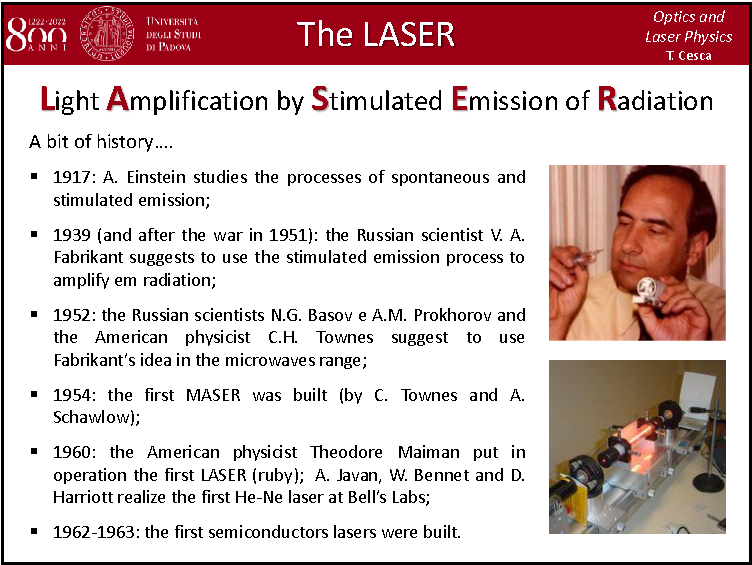
\includegraphics[page=1,width=1\textwidth]{../lessons/pdf_file/07_lecture.pdf}
\end{minipage}
\hspace{0.3cm}\vspace{0.3cm}
\begin{minipage}[c]{0.47\linewidth}

Laser: idea of stimulated emission to amplify the radiation.

\end{minipage}

\subsubsection*{Slide 2}

\begin{minipage}[]{0.5\linewidth}
\centering
\includegraphics[page=2,width=1\textwidth]{../lessons/pdf_file/07_lecture.pdf}
\end{minipage}
\hspace{0.3cm}\vspace{0.3cm}
\begin{minipage}[c]{0.47\linewidth}

The main elements (indipendent on the kind of laser) are:
\begin{itemize}
\item \textbf{active medium}: material which is able to amplify the radiation which is able to obtain stimulated emission. A cascade of photons is obtained: the medium is acting as an \emph{amplifier}.

\item \textbf{pumping system}: the material needs to be in \emph{out of equilibrium condition}.

\item \textbf{cavity}: the laser should have a feedback process in which the photons produced within the active medium can start oscillatating back and forth inside an \emph{optical cavity} to obtain more photons. The simple cavity is composed by two mirrors. At least, one of the two mirror should have reflectivity less than 100 $\%$ to extract the beam. This is called \textbf{outcoupling mirror}.

\end{itemize}

\end{minipage}

\subsubsection*{Slide 3}

\begin{minipage}[]{0.5\linewidth}
\centering
\includegraphics[page=3,width=1\textwidth]{../lessons/pdf_file/07_lecture.pdf}
\end{minipage}
\hspace{0.3cm}\vspace{0.3cm}
\begin{minipage}[c]{0.47\linewidth}

Main properties of a laser beam which make a laser a very specific light source.

\end{minipage}

\newpage

\subsubsection*{Slide 4}

\begin{minipage}[]{0.5\linewidth}
\centering
\includegraphics[page=4,width=1\textwidth]{../lessons/pdf_file/07_lecture.pdf}
\end{minipage}
\hspace{0.3cm}\vspace{0.3cm}
\begin{minipage}[c]{0.47\linewidth}

Typically, lasers emit at one specific wavelength. \textbf{Monochromaticity} is related to this.

The process of stimulated emissions will occur between two energy levels. The constraint about the frequency is related to the difference of energetic levels.

Moreover, the active medium is inside the optical cavity. Only the frequencies that are in resonance with the cavity can propagate, all the other will be damped in few steps.

These are the reasons of monochromaticity.

\end{minipage}

\subsubsection*{Slide 5}

\begin{minipage}[]{0.5\linewidth}
\centering
\includegraphics[page=5,width=1\textwidth]{../lessons/pdf_file/07_lecture.pdf}
\end{minipage}
\hspace{0.3cm}\vspace{0.3cm}
\begin{minipage}[c]{0.47\linewidth}

The reason of \textbf{directionality} is related to the presence of the optical cavity. Typically they are open cavities, all the modes that can propagate along the cavity axis are sustained by the cavity, otherwise they are lose.
In this slide, one the top, we can see an image example.
So, only the rays close to the axis of the cavity remains, this is why laser has an high directionality.

The simplest cavity is the \textbf{Fabry-Perot}, but it is not too simple to align the beam.

\end{minipage}

\subsubsection*{Slide 6}

\begin{minipage}[]{0.5\linewidth}
\centering
\includegraphics[page=6,width=1\textwidth]{../lessons/pdf_file/07_lecture.pdf}
\end{minipage}
\hspace{0.3cm}\vspace{0.3cm}
\begin{minipage}[c]{0.47\linewidth}

\textbf{Brilliance} is the emitted power per unit of surface (which is the \emph{intensity}) and unit of solid angle.

Given the high directionality, also a laser with limited power, can have a brilliance several order higher than conventional light sources.

\end{minipage}

\newpage

\subsubsection*{Slide 7}

\begin{minipage}[]{0.5\linewidth}
\centering
\includegraphics[page=7,width=1\textwidth]{../lessons/pdf_file/07_lecture.pdf}
\end{minipage}
\hspace{0.3cm}\vspace{0.3cm}
\begin{minipage}[c]{0.47\linewidth}

Let us compare the brilliance of laser wrt a conventional source.

The intensity of a black body can be computed with the \textbf{stefan-boltzmann's law}. So, the convential intensity is of the order \( \sim 10^4 \) K, while for laser is \( \sim 10^6-10^7 \) K.

\end{minipage}

\subsubsection*{Slide 8}

\begin{minipage}[]{0.5\linewidth}
\centering
\includegraphics[page=8,width=1\textwidth]{../lessons/pdf_file/07_lecture.pdf}
\end{minipage}
\hspace{0.3cm}\vspace{0.3cm}
\begin{minipage}[c]{0.47\linewidth}

Laser beam have an high degree of both \textbf{spatial and temporal coherence}.

Let us consider two points. If the phase coherence is null at every time, there is perfect coherences between the two points. If this happen for every point of a wavefront, there is \textbf{perfect} spatial coherence. In practice, a good degree of correlation is obtained for points within a given area: \textbf{partial} spatial coherence.


\end{minipage}

\subsubsection*{Slide 9}

\begin{minipage}[]{0.5\linewidth}
\centering
\includegraphics[page=9,width=1\textwidth]{../lessons/pdf_file/07_lecture.pdf}
\end{minipage}
\hspace{0.3cm}\vspace{0.3cm}
\begin{minipage}[c]{0.47\linewidth}

The \textbf{coherence length} is the propagation distance within which it is mantained a given degree of spatial coherence.

A theorem staes that coherence area is related to the square power of the distance of the source. Hence, wavefronts tend to smooth-out going far away from the source.

Lasers are the sources with the highest spatial coherence.

\end{minipage}

\subsubsection*{Slide 10}

\begin{minipage}[]{0.5\linewidth}
\centering
\includegraphics[page=10,width=1\textwidth]{../lessons/pdf_file/07_lecture.pdf}
\end{minipage}
\hspace{0.3cm}\vspace{0.3cm}
\begin{minipage}[c]{0.47\linewidth}

Let us consider the electric field at a given point at time \( t \) and \( t + \tau  \). If the phase difference between the two electric field at time \( t \) and \( t + \tau  \) is the same for every \( t \), there is \textbf{temporal coherence within time} \( \pmb{\tau } \).

If this happen for every \( \tau  \), we have \textbf{perfect} temporal coherence.

If it happen only for \( \tau  \) in an interval, we have \textbf{partial} temporal coherence.

In this first example, the coherence time is infinite.


\end{minipage}

\subsubsection*{Slide 11}

\begin{minipage}[]{0.5\linewidth}
\centering
\includegraphics[page=11,width=1\textwidth]{../lessons/pdf_file/07_lecture.pdf}
\end{minipage}
\hspace{0.3cm}\vspace{0.3cm}
\begin{minipage}[c]{0.47\linewidth}

In this case, we have a finite coherence time.

\end{minipage}

\subsubsection*{Slide 12}

\begin{minipage}[]{0.5\linewidth}
\centering
\includegraphics[page=12,width=1\textwidth]{../lessons/pdf_file/07_lecture.pdf}
\end{minipage}
\hspace{0.3cm}\vspace{0.3cm}
\begin{minipage}[c]{0.47\linewidth}

Spatial and temporal coherence are \textbf{independent concepts}:

\begin{itemize}
\item spatial coherence is associated with the wave properties \textbf{transverse} to the direction of propagation.

\item temporal coherence is associated with the properties \textbf{along} the direction of propagation.

\end{itemize}

The coherence time is inversionally proportional to the bandwidth, so that you can write it in term of wavelngth. So, \emph{the more monochromatic is your beam, the larger is the coherent time}.

Atomic sources have a very high degree of monochromaticity, so that you can obtain a very high degree of temporal coherence. Regarding spatial coherence, there are no sources that can be competitive with any laser beam!

\end{minipage}

\subsubsection*{Slide 13}

\begin{minipage}[]{0.5\linewidth}
\centering
\includegraphics[page=13,width=1\textwidth]{../lessons/pdf_file/07_lecture.pdf}
\end{minipage}
\hspace{0.3cm}\vspace{0.3cm}
\begin{minipage}[c]{0.47\linewidth}

This is not an intrinsic property of any laser, but it can be obtained by using special techniques as \textbf{mode-locking}.

Ultra-short puls is the counterpart of monochromaticity.

\end{minipage}

\subsubsection*{Slide 14}

\begin{minipage}[]{0.5\linewidth}
\centering
\includegraphics[page=14,width=1\textwidth]{../lessons/pdf_file/07_lecture.pdf}
\end{minipage}
\hspace{0.3cm}\vspace{0.3cm}
\begin{minipage}[c]{0.47\linewidth}

For the time, we simplify the description with a two level system: \textbf{first} and \textbf{second} \textbf{level}.

The two levels have a \textbf{population}: number of atom per unit of volume at a given energy level.

The energy difference is related to the frequency of emission. If we have a non negligible population in the upper level, you will have the spontaneous decay of the atom from upper to lower level and consequently an emission of photons.

We can write the change in population over time with \textbf{Einstein coefficient} related to spontaneous emission between 2 and 1 (first term).
There are other process that reduce the population, as emission toward other levels (second term). We have to sum up all these process. We have other \emph{non radiative processes} (without the emission of photons) (third term).
We can define a \textbf{total lifetime} \( \tau  \) for the energy level 2.

\end{minipage}

If we solve the rate equation, we obtain an exponential decay. The population of the upper level is decaying with a lifetime constant which is the total lifetime of the upper level (not only the spontaneous one!).

\subsubsection*{Slide 15}

\begin{minipage}[]{0.5\linewidth}
\centering
\includegraphics[page=15,width=1\textwidth]{../lessons/pdf_file/07_lecture.pdf}
\end{minipage}
\hspace{0.3cm}\vspace{0.3cm}
\begin{minipage}[c]{0.47\linewidth}

The power is an exponential decay, which has a time constant which is the total lifetime of the upper energy level.

In a lifetime experiment you are measuring the total lifetime!

\end{minipage}

\subsubsection*{Slide 16}

\begin{minipage}[]{0.5\linewidth}
\centering
\includegraphics[page=16,width=1\textwidth]{../lessons/pdf_file/07_lecture.pdf}
\end{minipage}
\hspace{0.3cm}\vspace{0.3cm}
\begin{minipage}[c]{0.47\linewidth}

The \textbf{fluorescente quantum yield} is the number of photons corresponding to the energy of the transition divided by the number of atoms in the energy level. This take into account only for the spontaneous emission process since you have to consider other processes. This is given by the ration between the total lifetime and the spontaneous lifetime. This is the probability of getting spontaneous emission of photons in this transition wrt the other processes that may occur.

\end{minipage}

\subsubsection*{Slide 17}

\begin{minipage}[]{0.5\linewidth}
\centering
\includegraphics[page=17,width=1\textwidth]{../lessons/pdf_file/07_lecture.pdf}
\end{minipage}
\hspace{0.3cm}\vspace{0.3cm}
\begin{minipage}[c]{0.47\linewidth}

Another process to take into account is \textbf{absorbtion}. Let us shine a beam with an energy and we match the energy of the transition. The energy can be absorbed and we have an equation which describe this process.

The population on the lower energy lever is decreasing over time. The spontaneous transition rate was depending only on the specific transition we were considering. Instead, the absorbition rate (absorbtion transition on the unit of time) depend on the number of photons that you are shining.
We have the \textbf{Einstein's coefficient for absorption} multiplied by \( n ( \nu ) \) (number of photons per unit of frequency), multiplied by the energy of the transition. Hence, we obtain the Einstein coefficient which multiply the energy density \( \rho (\nu ) \). We can write it as a function of the \textbf{absorption cross-section} for the \textbf{photon flux}.
So, the absorption depends on the flux of photons we are shining.

\end{minipage}

\subsubsection*{Slide 18}

\begin{minipage}[]{0.5\linewidth}
\centering
\includegraphics[page=18,width=1\textwidth]{../lessons/pdf_file/07_lecture.pdf}
\end{minipage}
\hspace{0.3cm}\vspace{0.3cm}
\begin{minipage}[c]{0.47\linewidth}

We are in a situation in which the population of 2 is non negligible and we shine the system with the energy of the transition.  \textbf{Stimulated emission} can be obtained: atoms are forced to decay from the level 2 to 1 with emission of photon related to the transition. We obtai two photons: the one we are shining and the second related to the transition induced.

The more transition that you induce, the more the larger of photons that you stimulate to produce.

The variation over time of the population of the energy level 2 is given by minus a stimulated emission rate for the population.

\end{minipage}

The \textbf{stimulated emission rate} does not depend only on the transition, but also on the flux of photons that you are shining.
The \( B_{21} \) is the \textbf{Einstein's coefficient for stimulated emission}. As for absorption we have a parameter which depend on the specific transition you are considering \( \sigma
_{21} \) but also the photon flux \( F \).

In the following, we will use rate equation for describing processes (semi-classical approach).

\end{document}
